%%%%%%%%%%%%%%%%%%%%%%%%%%%%%%%%%%%%%%%%%%%%%%%%%%%%%%%%%%%%%%%%%%%%%
%% TODO: 
%% -- The tail part of the lecture after Cost has not been 
%%    updated in a while.
%%
%% -- Complete the climbing DAG example in TopSort section.
%% -- Talk about DFG as graph search by using a stack for a frontier.
%% -- The last two section are not fully integrated (missing SPARC
%% -- definitions, etc)
%%%%%%%%%%%%%%%%%%%%%%%%%%%%%%%%%%%%%%%%%%%%%%%%%%%%%%%%%%%%%%%%%%%%%%
\chapter{Graph Search}
\label{ch:graph-search}



\begin{notesonly}
\paragraph{BFS lecture outline.}
\begin{enumerate}
\item Reachability and shortest paths
\item Vertex Hopping: visit vertices and edges
\item Ask: reachability with vertex hopping
\item Motivate: graph search
\item Write code for graph search
\item BFS, define by levels \exref{bfs::levels-simple}
\item Ask: how to modify graph search to perform BFS
\item Give BFS code
\item Define $X_i$ as the set of vertices visited before round $i$.
\item Prove \lemref{bfs::main}
\item Reachability solve with BFS
\item Termination of BFS, total number of rounds.
\item BFS with distance
\item Shortest-paths tree = BFS Tree, \exref{bfs::bfs-trees}
\item Cost of BFS with trees and st sequences
\item Leave the code with st sequences as exercise.
\end{enumerate}


\paragraph{DFS lecture outline.}
\begin{enumerate}
\item Draw the climbing DAG
\item DAG has no cycles and is  a dependency graph.
\item Talk about how the climber uses thes DAG
\item Do a demo
\item Define the topological sort problem 
\item Discuss how BFS does not work.
\item Intro DFS
\item Give examples
\item Talk about why DFS is a graph search, define frontier as a
  stack.  THIS MIGHT NEED TO BE WORKED OUT MORE CAREFULLY THAN IT IS
  IN THE NOTES.

\item Talk about DFS numbers.
\item Implement TopSort with DFS.
\item Cost bounds
\end{enumerate}

\end{notesonly}
 
The term \defn{graph search} or \defn{graph traversal} refers to a class
of algorithms that systematically explore the vertices and edges of a
graph.  Graph-search algorithms can be used to solve many interesting
problems on graphs, or compute many interesting properties of graphs; they are indeed at the heart of many
graph algorithms.
% 
In this chapter, we introduce the concept of a graph search,
describing a general algorithm for it.
%
We then consider further specializations of this general algorithm,
specifically the breadth-first search (BFS), depth-first search (DFS),
and priority-first search (PFS) algorithms, each of which is
particularly useful in computing certain properties of graphs.   
Graph search can be applied to both directed and undirected graphs.

As an example of what graph search may be used for consider the
following problem.  We say that a vertex $v$ is \defn{reachable} from
$u$ in the graph $G$ (directed or undirected) if there is a path from
$u$ to $v$ in $G$.  Then we have:
\begin{problem}[The Graph Reachability Problem]
For a graph $G = (V,E)$ and a vertex $v \in V$, return all vertices $U
\subseteq V$ that are reachable from $v$.
\end{problem}
Another problem
we may wish to solve with graph search is to determine the shortest 
path from a vertex to all other vertices.     This is covered in the
next chapter.

As the problems above suggest, a graph search usually starts at a
specific vertex, and also sometimes at a set of vertices.  We refer to
such a vertex (vertices) as the \defn{source} vertex (vertices). 
Graph search then searches out from this source (or these sources) and
\defn[visit (in graph search)]{visits} neighbors of vertices that have already been visited.
%
To ensure efficiency, graph search algorithms usually keep track of
the vertices that have already been visited to avoid visiting a
vertex for a second time.    We will refer to these as the
\defn{visited set} of vertices, and often denote them with the
variable $X$.
Since we only visit un-visited neighbors of the visited set it can be useful to keep track of all such vertices.
We will refer to these vertices as the frontier.   More formally:

\begin{notesonly}
Throughout this chapter and more generally in this book, we use a
special syntax for loops.

\begin{syntax}
We use the syntax
~\\
\begin{lstlisting}
$(X_1, \ldots, X_k)$ = 
  start $(v_1, \ldots, v_k)$ and
  while $e_c$ do
    $e_w$
\end{lstlisting}
as syntactic sugar for 
\begin{lstlisting}

loop $(X_1, \ldots, X_k)$ = 
  if $e_c$ then
    let $e_w$ in loop $(X_1, \ldots, X_k)$ end
  else
   $(X_1, \ldots, X_k)$ 

$(X_1, \ldots, X_k)$ = loop $(v_1, \ldots, v_k)$. 
\end{lstlisting}

\end{syntax}
\end{notesonly}

%% Begin: vertex hopping
\begin{notesonly}
\paragraph{Vertex Hopping.}

As a warm-up, let start with a technique that we call {\em vertex
  hopping}.  As we will see vertex hopping is not helpful in many
cases but it can offer a good starting point in appreciating some
intricacies of graph search.
%
The idea behind vertex hopping is repeatedly select some set of
vertices to visit, visit them, and continue until all vertices are
visited.  More precisely, vertex hoping can be expressed as follows

\begin{algorithm}[Vertex Hopping]
vertexHopper (G = (V,E), s) = 

\begin{lstlisting}
vertexHop $(G = (V,E), s)$ =
  visit source $s$

  let $X$ = 
    start $\{s\}$ and
    while $X \not= V$ do
      choose $U$ such that $U \subseteq V \setminus X$
      visit the vertices in $U$
      visit the out-edges of the vertices in $U$
      $X = X \cup U$    
\end{lstlisting}
\end{algorithm}

The algorithm starts by visiting the source vertex and uses the set
$X$ to keep track of all the vertices that it has thus far visited.
%
At each step (iteration of the while loop), the algorithm
non-deterministically selects a set of un-visited vertices and visits
them.
%
Note that the algorithm as expressed is naturally parallel: we can
visit many vertices at the same time.  
%

\begin{question}
When the algorithm terminates, does it visit all the edges? 
\end{question}
%
Since the algorithm visits all the out-edges of a vertex when it
visits the vertex and since it visits all the vertices, the algorithm
also visits all the edges.

As an example of how we might use vertex hopping to solve a graph
problem, let's consider reachability.  
%
\begin{question}
Can you solve the reachability problem using vertex hopping?
\end{question}
%
We can solve the reachability problem by keeping a table mapping each
visited vertex to the set of vertices reachable from it.  When 
we visit a vertex $u$, we extend the table by finding all the vertices
that can reach $u$ and extending their reach by adding $v$ for every
edge $(u,v)$.


\begin{question}
Is this algorithm efficient? 
\end{question}
%
Unfortunately, this algorithm is not efficient.  In reachability, we
are interested in finding out whether a particular vertex is reachable
from another. This algorithm is building the full the reachability
information for all vertices.
%
\begin{question}
Can you see why vertex hopping is not effective for reachability
computations?  
\end{question}
%

The problem is that the algorithm is not taking advantage of the
structure of the graph: it nondeterministically jumps around the graph
to visit vertices without following paths in the graph.  As we will
see in later, vertex hopping, especially its parallel version, can be
useful in some applications but for problems such as reachability, the
algorithm is not able to recover efficiently the path information.

\end{notesonly}
%% End: vertex hopping

%Since many interesting properties of graphs involves paths,
%graph-search algorithms that we will consider here will visit
%(explore) the vertices in the graph by following paths.  
%
\begin{question}
Can you see how we can build on vertex hopping to visits paths?  
\end{question}
%
%To do this efficiently, graph search algorithms usually maintain a
%set of frontier vertices, which are not yet visited but are adjacent to
%visited vertices, and visit a vertex only when it is in the frontier. %
%
\begin{definition}
For a graph $G = (V,E)$ and a visited set $X \subset V$, the
\defn{frontier set} is the set of un-visited out neighbors of 
of $X$, i.e. the set $N^+_G(X) \setminus X$.
\end{definition}
Recall that $N^+_G(v)$ are the outgoing neighbors of  
the vertex $v$ in the graph $G$, and $N^+_G(U) = \bigcup_{v \in U} 
N^+_G(v)$ (i.e., the union of all out-neighbors of $U$).
 We often denote the frontier set with the variable $F$.
%
Assuming we start at a single source vertex $s$,
we can now write a generic graph-search algorithm as follows.
%
\begin{algorithm}[Graph Search]~
\label{alg:graph-search::graph-search}
\begin{lstlisting}
graphSearch $(G,s)$ =
  let
   $(X, F)$ = 
     start  $(\{\}, \{s\})$ and
     while $(|F| > 0)$ do
      choose $U \subseteq F$ such that $|U| \geq 1$ @\label{line:gs::choose}@
      visit $U$
      $X$ = $X \cup U$     % Add newly visited vertices to $X$   
      $F$ = $N^+_G(X) \setminus X$  % The next frontier, i.e. neighbors of $X$ not in $X$
  in $X$ end
\end{lstlisting}
\end{algorithm}

The algorithm starts by initializing the visited set of vertices $X$
with the
empty set and the frontier with the source $s$.  It then proceeds in a
number of {\em rounds}, each corresponding to an iteration of
the while loop.  At each round, the algorithm selects a subset $U$ of
vertices in the frontier (possibly all), visits them, and updates the visited and the
frontier sets.   Note that when visiting the set of vertices $U$, we can
usually visit them in parallel.      
The algorithm terminates when there are no more
vertices to visit---i.e., the frontier is empty. 
%
\begin{question}
Does the algorithm visit all the vertices in the graph?
\end{question}
%
This does not mean that it visits all the vertices: vertices that are
not reachable from the source will never be visited by the algorithm.
%
In fact, the function \ttt{graphSearch} returns exactly the set of vertices
that are reachable from the source vertex $s$.    Hence
\ttt{graphSearch} solves the reachability problem, and this
is true for any choice of $U$ on line~\ref{line:gs::choose}.
%
In many applications of graph search, we keep track of other
information in addition to the reachable vertices.

Since the function \ttt{graphSearch} is not specific about the set of
vertices to be visited next, it can be used to describe many different
graph-search techniques.  In this chapter we  consider three methods
for selecting the subset, each leading to a specific
graph-search technique.  Selecting all of the vertices in the frontier
leads to breadth-first search.  Selecting the single most recently
``seen'' vertex from the frontier leads to depth-first search (when
visiting a vertex we ``see'' all its neighbors).  Selecting the
highest-priority vertex (or vertices) in the frontier, by some
definition of priority, leads to priority-first search.  Note that
breadth-first search is parallel since it can visit many vertices at
once (the whole frontier), while depth-first-search is sequential
since it only visits one vertex at a time.

Since graph search always visits an out-neighbor of the visited set,
we can associate every visited vertex with an in-neighbor from which
it was visited.  When a vertex is visited there might be many
in-neighbors that have already been visited, so we have to choose one.
The mapping of vertices to their chosen in-neighbor defines a tree
over the reachable vertices with the source $s$ as the root.  In
particular the parent of each vertex is its in-neighbor that is chosen
when visited.   The source $s$ has no parent and is therefore the
root.  This tree is referred to as the \defn{graph search
  tree}.  We will see that it is useful in various applications.

%% Note that graph-search effectively follows paths because it only
%% visits a vertex $u$ from one of its incoming edges.  This does not
%% mean that the algorithm always follows a single path as far is it can
%% and then switches to another path.  Rather, the algorithm is extending
%% a set of paths simultaneously and in an interleaved fashion.

\section{Breadth-First Search (BFS) \defn[BFS (breadth-first
search)]{}}
\label{sec:bfs}
\label{sec:gs::bfs}

\newcommand{\bfs}{\ttt{BFS}}

The \defn{breadth-first search} (BFS) algorithm is a particular graph-search algorithm that
can be applied to solve a variety of problems.  Beyond solving the
reachability problem, it can be used to find the shortest (unweighted)
path from a given vertex to all other vertices, determining if a graph
is bipartite, bounding the diameter of an undirected graph,
partitioning graphs, and as a subroutine for finding the maximum flow
in a flow network (using Ford-Fulkerson's algorithm).  As with the
other graph searches, BFS can be applied to both directed and
undirected graphs.

To understand how BFS operates, consider a graph $G = (V,E)$ and a
source vertex $s \in V$.  Define the \defn[level (in breadth-first
search)]{level} of a vertex $v \in V$ as the shortest distance from
$s$ to $v$, that is the number of edges on the shortest path
connecting $s$ to $v$ in $G$, denoted as $\delta_G(s,v)$ (we often drop the
$G$ in the subscript when it is clear from the context).

Breadth first search (BFS) starts at the given \emph{source}
vertex $s$ and explores the graph outward in all directions in
increasing order of levels. It first visits all the vertices that are
the out-neighbors of $s$ (i.e. have distance $1$ from $s$, and hence
are
on level $1$), and then
continues on to visit the vertices that are on level $2$ (have distance $2$ from $s$),
then level $3$, and so on.

\begin{example}
\label{ex:bfs::levels-simple}
A graph and its levels illustrated.  BFS visits the vertices on levels
0, 1, 2, and 3 in that order.   
\vspace{-.1in}
\begin{center}
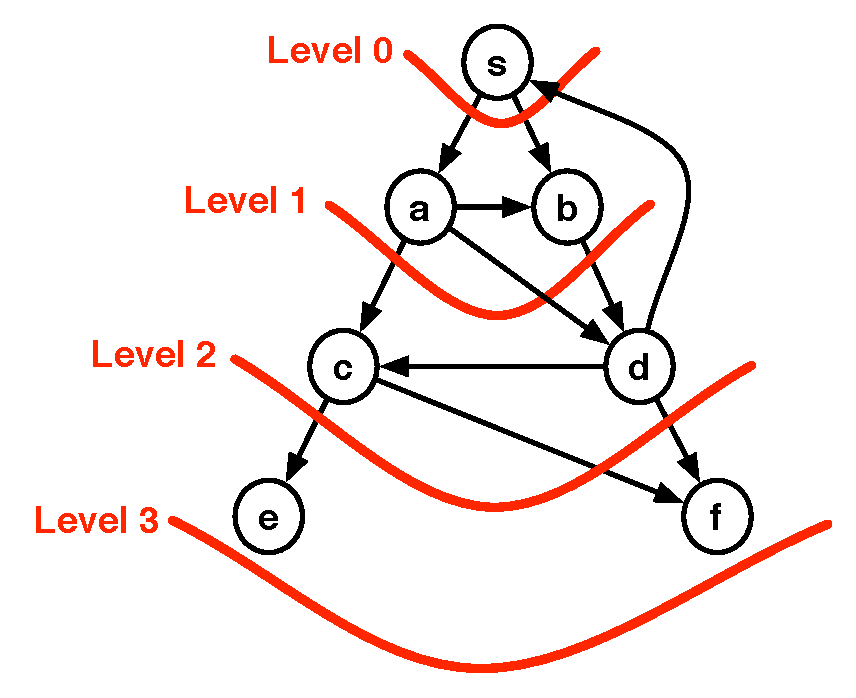
\includegraphics[width=2.6in]{graph-search/directed-graph-levels}
\end{center}
\vspace{-.1in}
Since $f$ is on level $3$, we have that $\delta(s,f) = 3$.   In fact
there are three shortest
paths of equal length: $\cseq{s,a,c,f}$, $\cseq{s,a,d,f}$ and $\cseq{s,b,d,f}$.
\end{example}

%% Begin: BFS is graph search
\begin{notesonly}
BFS is a graph-search algorithm in a precise sense: it can be
expressed as a specialization of the graph search algorithm
(\algref{graph-search::graph-search}).
%
To understand the structure of BFS, it is instructive to go through
the exercise of convincing ourselves that this is the case.
%
One way to show that BFS is an instance of graph-search is to specify
the way we select the vertices to be visited next (the set $U$).
%
\begin{question}
Can specify the selection of vertices to visit in
\algref{graph-search::graph-search} to make sure that the vertices are
visited in breadth-first order?
\end{question}
%

We can achieve this by enriching the frontier with levels, for
example, by tagging each vertex with its level, and selecting, at each
round, the vertices at the current level to visit.  But this would
work only if we can make sure to insert all vertices ``in time'' to
the frontier set, i.e., all vertices at level $i$ should be inserted
before we get to that level.
%
\begin{question}
How can we determine the set of vertices at level $i$?
\end{question}
%
Note that since the vertices at level $i$ are all connected to
vertices at level $i-1$ by one edge, we can find all the vertices at
level $i$ when we find the outgoing neighbors of level-$i-1$ vertices.
%
\begin{question}
Is the set of vertices that are at level $i$ equal to the vertices
reachable from level-$i-1$ vertices by one edge?
\end{question}
%

The outgoing neighbors may be at level $i$ or less. But since we have
visited all the vertices at level less than $i$, the un-visited
vertices will be exactly the level-$i$ vertices.

\begin{exercise}
Based on the discussion, complete the specification of BFS and modify  
\algref{graph-search::graph-search} to perform BFS.
\end{exercise}

\end{notesonly}
%% End: BFS is graph search

As mentioned in the introduction, the BFS-algorithm is a specialization of the
graph-search algorithm (\algref{graph-search::graph-search}) for which
all frontier vertices are visited on each round.  
The algorithm can thus be defined as follows:

\begin{algorithm}[BFS: reachability and radius]~
\label{alg:bfs}
\begin{lstlisting}
BFSReach $(G = (V,E),s)$ =
  let
    $(X, F, i)$ = 
      start $(\{\}, \{s\}, 0)$ and
      while $(|F| > 0)$ 
        invariant: $X = \csetf{u \in V}{\delta_G(s,u) < i} \wedge$
                   $F = \csetf{u \in V}{\delta_G(s,u) = i}$
        $X$ = $X \cup F$        
        $F$ = $N^+_G(F) \setminus X$  
        $i$ = $i + 1$          
  in $(X,i)$ end
\end{lstlisting}
\end{algorithm}

In addition to the visited set $X$ and frontier $F$ maintained
by the general graph search, the algorithm maintains the level $i$.
%
It searches the graph level by level, starting at level $0$ (the
source $s$), and visiting one level on each round of the while loop.
%
We refer to all the vertices visited before level (round) $i$ as $X_i$.
%
Since at level $i$ we visit vertices at a distance $i$, and since we
visit levels in increasing order, the vertices in $X_i$ are exactly
those with distance less than $i$ from the source.
%

At the start of round $i$ the frontier $F_i$ contains all
un-visited neighbors of $X_i$, which are the vertices in the graph with
distance exactly $i$ from $s$.
% 
In each round, the algorithm visits all the vertices in the frontier
and marks newly visited vertices by adding the frontier to the visited
set, i.e, $X_{i+1} = X_i \cup F_i$.  
%
To generate the next set of frontier vertices, the algorithm takes the
neighborhood of $F$ and removes any vertices that have already been
visited, i.e., $F_{i+1} = N^+_G(F) \setminus X_{i+1}$. 
%
Algorithm~\ref{alg:bfs} just keeps track of the visited set $X$, the frontier
$F$,
and the level $i$, but, as we will see, in general BFS-based algorithms can keep
track of other information.


\begin{example}
\label{ex:bfs::levels}
The figure below illustrates the BFS visit order by using overlapping
circles from smaller to larger.  Initially, $X_0$ is empty and $F_0$
is the single source vertex $s$, as it is the only vertex that is a
distance 0 from $s$.  $X_1$ is all the vertices that have distance
less than 1 from $s$ (just $s$), and $F_1$ contains those vertices
that are on the middle ring, a distance exactly 1 from $s$ ($a$ and
$b$).  The outer ring contains vertices in $F_2$, which are a distance
2 from $s$ ($c$ and $d$).  The neighbors $N_G(F_1)$ are the central
vertex $s$ and those in $F_2$.  Notice that vertices in a frontier can
share the same neighbors (e.g., $a$ and $b$ share $d$), which is why
$N_G(F)$ is defined as the \emph{union} of neighbors of the vertices
in $F$ to avoid duplicate vertices.
  
\begin{center}
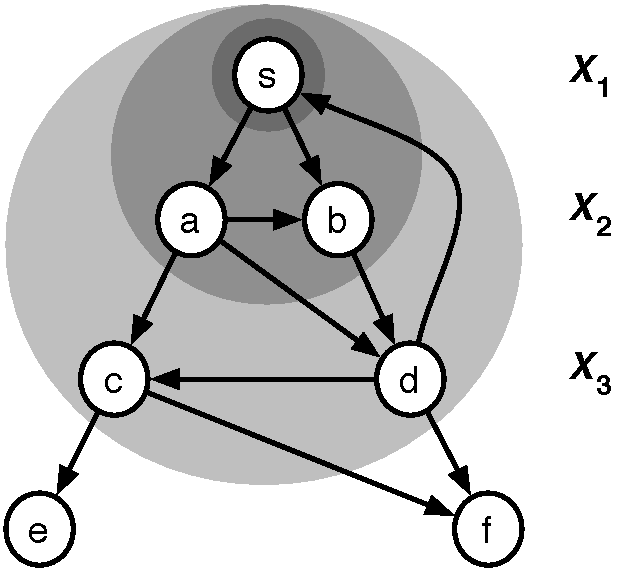
\includegraphics[width=2.25in]{graph-search/directed-graph-bfs}
\end{center}
\end{example}


To prove that the algorithm is correct we need to prove the invariant
that is stated in the algorithm.  

\begin{lemma}
\label{lem:bfs::main}
In \ttt{BFSReach} the invariants $X = \csetf{v \in V_G}{\delta_G(s, v) < i}$
and $F = \csetf{v \in V_G}{\delta_G(s, v) = i}$ are maintained.
\end{lemma}
\begin{proof}
This can be proved by induction on the level $i$.  For the base case
$i = 0$, and we have $X_0 = \cset{}$ and $F_0 = \cset{s}$.
%
This is true since no vertex has distance less than 0 from $s$ and
only $s$ has distance 0 from $s$.  For the inductive step, we assume
the properties are correct for $i$ and want to show they are correct for $i+1$.  For
$X_{i+1}$, the algorithm takes the union of all vertices at distance
less than $i$ ($X_i$) and all vertices at distance exactly $i$
($F_i$). So $X_{i+1}$ is exactly the vertices at a distance less than
$i+1$.  
%
For $F_{i+1}$, the algorithm takes all neighbors of $F_i$ and
removes the set $X_{i+1}$.  Since all vertices $F_i$ have distance $i$
from $s$, by assumption, then a neighbor $v$ of $F$ must have
$\delta_G(s,v)$ of no more than $i+1$.  
%
Furthermore, all vertices of distance $i+1$ must be reachable from a
vertex at distance $i$.  Therefore, the out-neighbors of $F_i$ contain all
vertices of distance $i+1$ and only vertices of distance at most
$i+1$.  When removing $X_{i+1}$ we are left with all vertices of
distance $i+1$, as needed.
\end{proof}

To see that the algorithm returns all reachable vertices, note that if
a vertex $v$ is reachable from $s$, then there
is a path from $s$ to $v$ and the vertices on that path have
have distances $0, 1, 2, 3, \ldots, \delta(s,v)$.   
Therefore for all rounds of \ttt{BFSReach} where $i \leq \delta(s,v)$ the frontier
$F$ is non empty, and the algorithm continues to the next round,
eventually reaching $v$ on round $\delta(s,v)$, which is at most $|V|$.
Note that the algorithm also returns $i$, which is the maximum
distance from $s$ to any reachable vertex in $G$.

%
\begin{question}
After how many rounds will the algorithm terminate?
\end{question}
%

\begin{exercise} 
In general, from which frontiers could the vertices in $N_G(F_i)$ come
when the graph is undirected?  What if the graph is directed?
\end{exercise}

\section{Shortest Paths and Shortest-Path Trees}

Thus far we have used BFS for reachability.  As you might have
noticed, however, our \ttt{BFSReach} algorithm is effectively
calculating the distance to each of the reachable vertices as it goes
along since all vertices $v$ that are visited on level $i$ have
$\delta(s,v) = i$.       But, the algorithm does not store this
information.     
It is relatively straightforward to extend BFS to keep track
of the distances.
For example the following algorithm takes a graph and a source and 
returns a table mapping every reachable vertex $v$ to $\delta_G(s,v)$.
\begin{algorithm}[BFS-based Unweighted Shorted Paths]~
\label{alg::bfsdistance}
\begin{lstlisting}
BFSDistance $(G,s)$ = 
  let 
    $(X,F,i)$ = 
      start $(\{\},\{s\},0)$ and
      while $(|F| > 0)$ 
        $X$ = $X \cup \{v \mapsto i : v \in F\}$
        $F = N^+_G(F) \setminus \ttt{domain}(X)$
        $i$ = $i + 1$          
  in $(X,i)$ end
\end{lstlisting}
\end{algorithm}
In the algorithm the table $X$ is used both to keep track of the
visited vertices and for each of these vertices to keep its distance
from $s$.  When visiting the vertices in the frontier we simply add
them to $X$ with distance $i$.

Sometimes in addition to the shortest distance to each vertex from
$s$, it might be useful to know a path (i.e. the vertices along the
path) which has that distance.  For example if your favorite map
program told you it was 2.73 miles to your destination, but did not
tell you how to get there it would not be too useful.  With hardly any
additional work it turns out we can generate a data structure during
BFS that allows us to quickly extract a shortest path from $s$ to any
reachable vertex $v$.  The idea is to generate a graph-search tree, as
defined in the introduction of this chapter---i.e., the parent of each
vertex $v$ is an in-neighbor of $v$ that was already visited when $v$
is visited.  When such a tree is generated with BFS, the path in the
tree from the root $s$ to a vertex $v$ is a shortest path from $s$ to
$v$.

To convince yourself the graph-search tree contains shortest paths,
consider a vertex $v$ visited at level $i$.  All in-neighbors already
visited when $v$ is visited must be at level $i-1$.  This is because
if they were at a lower level then $v$ would be visited earlier
(contradiction).  If they are at a higher level, then they are not yet
visited (contradiction again).  Therefore the parent $u$ of $v$ in the
tree must be exactly one closer to $s$.  The parent of $u$ must again
be one closer.  Therefore the path up the tree is a shortest path (at
least if we assume edges are unweighted).  We
therefore call a graph-search tree generated by BFS the unweighted
\defn[shortest-path tree (unweighted)]{shortest-path tree}.

We can represent a shortest-path tree with a table mapping each
reachable vertex to its parent in the tree.
%
Given such a shortest-paths tree, we can then compute the shortest path to a
particular vertex $v$ by walking in the tree from $v$ up to the
root $s$, and then reversing the order of the result.
%
Note that there could be more than one shortest-path tree, because
there can be multiple paths of equal length from the source to a vertex.  For example
\ref{ex:bfs::bfs-trees} shows two possible trees that differ while
still yielding the same shortest distances.

\begin{notesonly}
To find a parent for each vertex, we need to identify for each vertex
in the frontier $v \in F'$, one vertex $u \in F$ such that $(u,v) \in
E$.
%
More specifically, we can represent the visited vertices~$X$ and the
frontier~$F$ as tables that map vertices to their parents.  
%
In each round, we update visited table by merging the tables~$X$
and~$F$. Finding the next frontier requires tagging each neighbor with
its parent (via the edge leading to it) and then merging the results.
%
That is, for each $v \in F$, we generate a table $\{v \mapsto u : v
\in N^+(u)\}$ that maps each neighbor of $v$ back to $u$.  
%
%% This is quite a bit of detail.
When merging tables, we have to decide how to break ties since
vertices in the frontier might have the several (parent) neighbors; we
can break such ties arbitrarily, for example by taking the first
vertex.
\end{notesonly}

\begin{example}
\label{ex:bfs::bfs-trees}
An undirected graph and two possible BFS trees with distances
from~$s$. Non-tree edges, which are edges of the graph that are not on
a shortest paths are indicated by dashed lines.

\begin{center}
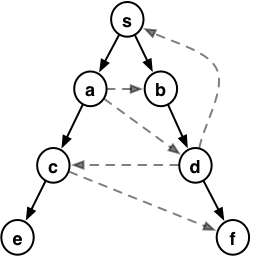
\includegraphics[width=1.9in]{graph-search/directed-graph-shortest-paths-1}
\hfill
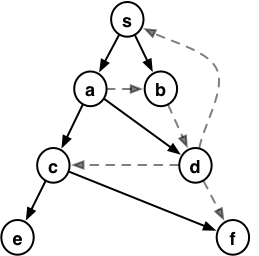
\includegraphics[width=1.9in]{graph-search/directed-graph-shortest-paths-2}
\end{center}

\end{example}

\begin{exercise}
  Modify Algorithm~\ref{alg::bfsdistance} to return a shortest-path
  tree represented as a table mapping each vertex to its parent.
  The source $s$ can map to itself.
\end{exercise}

The problem of finding the shortest path from a source to all other 
vertices (unreachable vertices are assumed to have infinite distance),
is called the \defn[single-source shortest path problem 
(unweighted)]{single-source shortest path problem}.  Here we are 
measuring the length of a path as the number of edges along the path. 
In the next chapter we consider shortest paths where each edge has a 
weight (length), and the shortest paths are the ones for which the sums of 
the weights are minimized.    Breadth-first search does not work for the 
weighted case. 



\section{Cost of BFS}

The cost of BFS depends on the particular representation that we
choose for graphs.  In this section, we consider two representations,
one using tree-based sets and tables, and the other using based on
single-threaded array sequences.  For a graph with $m$ edges and $n$
vertices, the first requires $O(m \log n)$ the second $O(m)$ work.
The span depends on the how many rounds the while loop makes, which
equals the largest distance of any reachable vertex from the source.
We will refer to as $d$.  The span with tree-based sets and tables is
$O(d \log^2n)$ (i.e. $O(\log^2 n)$ per level) and with array sequences
it is $O(d \log n)$ (i.e. $O(\log n)$ per level).

When analyzing the cost of BFS with either representation, a natural
method is to sum the work and span over the rounds of the algorithm,
each of which correspond to a single iteration of the while loop.  
%
In contrast with recurrence based analysis, this approach makes the
cost somewhat more concrete but can be made complicated by the fact
that the cost per round depends on the structure of the graph.  
%
We bound the cost for BFS observing that BFS visits each vertex at
most once, and since the algorithm only looks at a vertices out-edges
when visiting it, the algorithm also only uses every edge at most once.


\subsubsection{Cost with BST-Sets and BST-Tables}

Let's first analyze the cost per round.  In each round, the only
non-trivial work consists of the union $X \cup F$, 
%
the calculation of neighbors $N = N_G^+(F)$, and
%
the set difference $F' = N \setminus F$.
%
The cost of these operations depends on the number of out-edges of the
vertices in the frontier.  Let's use $\|F\|$
 to denote the number of
out-edges for a frontier plus the size of the frontier, i.e., $\|F\| =
\sum_{v \in F} (1 + d_G^+(v))$.  The costs for each round are then

\[
\begin{array}{lcc}
\toprule
  & \mbox{Work} & \mbox{Span} \\ 
\midrule

X \cup F & O(|F| \log n) & O(\log n) \\
N_G^+(F) & O(\|F\| \log n) & O(\log^2 n) \\
N \setminus X & O(\|F\| \log n) & O(\log n). \\
\bottomrule
\end{array}
\]

The first and last lines fall directly out of the tree-based cost
specification for the set ADT. 
%
 The second line is a bit more involved.  The union of out-neighbors
 is implemented as
\begin{lstlisting}[numbers=none]
let $N_G^+(F)$ = Table.reduce Set.Union $\cset{}$ (Table.restrict $G$ $F$)
\end{lstlisting}
Let $G_F = \ttt{Table.restrict}~G~F$. The work to find $G_F$ is $O(|F|
\log n)$.  
%
For the cost of the union, note that the set union results in a set
whose size is no more than the sizes of the sets unioned.  The total
work per level of reduce is therefore no more than $\|F\|$.  Since
there are $O(\log{n})$ such levels, the work is bounded by
%
\begin{align*}
\cwork{\ttt{Table.reduce}}\; \ttt{union}\; \{\}\; G_F)
& =  O\left(\log |G_F| \sum_{v \mapsto N(v) \in G_F} (1 + |N(v)|)\right)
\\
& = O\left(\log n \cdot \|F\|\right)
\\
\intertext{and span is bounded by}
%
\cspan{\ttt{reduce}\; \ttt{union}\; \{\}\;  G_F} & =  O(\log^2 n)
\end{align*} 
%
since each union has span $O(\log n)$ and the reduction
tree is bounded by $\log n$ depth.

%We can now calculate the span as the sum over all rounds, which gives
%us $O(d \log^2{n})$, where $d$ is the depth of the shortest path tree
%(longest path in the tree) or equivalently the total number of rounds.
%
%To calculate the work, we might want to find the sum of the work over
%all rounds, but unfortunately this is difficult because the work at
%each round depends on the frontier.
%

Focusing on a single round, we can see that the cost per vertex and
edge visited in that round is $O(\log n)$.  Furthermore we know that
every reachable vertex only appears in the frontier exactly once.
Therefore, all the out-edges of a reachable vertex are also processed
only once.  Thus the cost per edge $W_e$ and per vertex $W_v$
over the algorithm is the same as the cost per round.  We thus
conclude that $W_v = W_e = O(\log{n})$.
%
Since the total work is $W = W_v n + W_e m$ (recall that $n = |V|$ and
$m = |E|$), we thus conclude that
\begin{eqnarray*}
W_{BFS}(n,m,d) & = & O(n \log n + m \log n)\\
               & = & O(m \log n),~\mbox{and}
\\
S_{BFS}(n,m,d) & = & O(d \log^2 n).
\end{eqnarray*}
We drop the $n \log n$ term in the work since for BFS we cannot reach
any more vertices than there are edges.

Notice that span depends on $d$. In the worst case $d \in \Omega(n)$
and BFS is sequential.  Many real-world graphs, however, have low
diameter; for such graphs BFS has good parallelism.

\subsubsection{Cost with Single-Threaded Sequences}

Consider an enumerated graph $G = (V,E)$ where $V =
\{0,1,\ldots,n-1\}$.
%
%% As we shall show next, by using a particular representation for
%% enumerated graphs and by using single-threaded sequences to represent
%% the visited set, we can give an $O(m)$-work and $O(d \log n)$-span
%% implementation for BFS.
%
We can represent enumerated graphs as a sequence of sequences~$A$,
where $A[i]$ is a sequence representing the out-arcs of vertex $i$.
%
If the out-arcs are ordered, we can order them accordingly; if not,
we can choose an arbitrary order.

\begin{example}
The enumerated graph below can be represented as  
\[
\cseq{
\cseq{1,2},
\cseq{2,3,4},
\cseq{4},
\cseq{5,6},
\cseq{3,6},
\cseq{~},
\cseq{~}}.
\]


\begin{center}
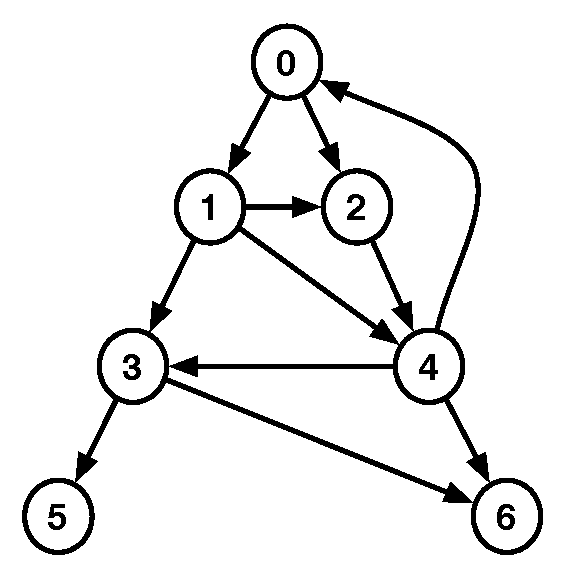
\includegraphics[width=1.9in]{graph-search/directed-graph-indexed}
\end{center}
\end{example}


This representation supports constant-work lookup operations for
finding the out-edges (or out-neighbors) of a vertex.  
%
Since the graph does not change during BFS, this representation
suffices for implementing BFS. 
%
In addition to performing lookups in the graph, the BFS algorithm also
needs to determine whether a vertex is visited or not by using the
visited set~$X$.  Unlike the graph, the visited set $X$ changes during
the course of the algorithm.  We therefore use a single-threaded
sequence of length $|V|$ to mark which vertices have been visited.  
%
By using \ttt{inject}, we can mark vertices in constant work per
update. 
%
For each vertex, we can use either a Boolean flag to indicate its
status, or the label of the parent vertex (if any).  The latter
representation can help up construct a BFS tree.

%%%%
%%%%
% In the BFS-tree the option $\cnone$ indicates the vertex has not been
% visited, and $\csome(v)$ indicates it has been visited and its parent
% is $v$.  Each time we visit a vertex, we map it to its parent in the
% BFS tree.  As the updates to this sequence are potentially small
% compared to its length, using an \texttt{stseq} is efficient.  On the
% other hand, because the set of frontier vertices is new at each level,
% we can represent the frontier simply as an integer sequence containing
% all the vertices in the frontier, allowing for duplicates.

The sequence-based BFS algorithm is shown in \algref{bfs::bfs-st}.
%
On entering the main loop, the sequence $\ttt{X}$ contains the parents
for both the visited and the frontier vertices instead of just for the
visited vertices. The frontier $F$ is represented a sequence
of vertices.
%
Each iteration of the loop starts by visiting the vertices in the
frontier (in this generic algorithm this includes no computation). 
%
Next, it computes the sequence $N$ of the neighbors of the vertices in
the frontier, and updates the visited set $X$ to map the vertices in
the next frontier to their parents. Note that a vertex in $N$ can have
several in-neighbors from $F$; the function \ttt{inject} selects one of
these as parent.
%
The iteration completes by computing the next frontier.  Since
\ttt{inject} guarantees a single parent, each vertex is included
at most once.
%

\begin{algorithm}[BFS Tree]~
\begin{lstlisting}
BFSTree $(G,s)$ =
  let 
    $X_0$ = STSeq.fromSeq $\cseq{\cnone : v \in \cseq{0,\ldots,|G|-1}}$
    $X$ = STSeq.update $X_0$ $(s,\csome{s})$

    (* Perform BFS. *)
    $(X,F)$ = 
      start $(X,\cseq{s})$ and
      while $(|F| > 0)$ 
        @(* Visit $F$ *)@
        @(* Compute next frontier and update visited. *)@
        $N =$ Seq.flatten $\cseq{\cseq{(u,\csome{v}) : u \in G[v] ~|~ X[u] = \cnone} : v \in F}$ @\label{line:bfs::flatten}@        
        $X = \ttt{STSeq.inject}~X~N$ @\label{line:bfs::inject}@        
        $F = \cseqf{u : (u,v) \in N}{X[u] = \csome{v}}$ @\label{line:bfs::F}@        
  in
    STSeq.toSeq $X$
  end
\end{lstlisting}
\label{alg:bfs::bfs-st}
\end{algorithm}

%% %\newcommand{\bfs}{\ttt{BFS}}
%% \begin{codel}
%% \cfun~\bfs = \newl
%% \clet\newl
%% ~~\cfun~\bfs' =\newl
%% ~~~~\cif~|F| = 0~\cthen~\ttt{stSeq.toSeq}~\ttt{XF}\newl
%% ~~~~\celse~\clet\newl[line:flatten]
%% ~~~~~~\cval~N = \ttt{flatten}\cseq{\cseq{(u,\csome(v)) : u \in G[v]} : v \in F}~~\cmark\ccomment{neighbors of the frontier}\newl[line:inject]
%% ~~~~~~\cval~\ttt{XF}' = \ttt{stSeq.inject}(N,~\ttt{XF})\ctab\ccomment{new parents added}\newl[line:F]
%% ~~~~~~\cval~F' = \cseqf{u : (u,v) \in N}{\ttt{XF}'[u] = v} \ctab\ccomment{remove duplicates}\newl
%% ~~~~\cin~\bfs'(\ttt{XF}',~F')~\cend \newl
%% ~~\cval~X_0 = \ttt{stSeq.toSTSeq}(\cseq{\cnone : v \in \cseq{0,\ldots,|G|-1}})\newl
%% \cin\newl
%% ~~\bfs'(\ttt{stSeq.update}(s,\csome(s),X_0),~\cseq{s})\newl
%% \cend
%% \end{codel}


All the work is done in \linereftwo{bfs::flatten}{bfs::inject},
and \lineref{bfs::F}.  Also note that the \ttt{STSeq.inject} on
\lineref{bfs::inject} is always applied to the most recent version. 
%
We can write out the following table of costs.

\[
\begin{array}{|c|c|c|c|c|}
\hline
 & \multicolumn{2}{c|}{$X$ : ST Sequence} &
\multicolumn{2}{c|}{$X$ : Sequence}
\\[2mm]
\hline
\mbox{Line} & \mbox{Work} & \mbox{Span} & \mbox{Work} & \mbox{Span} 
\\[2mm]
\hline
8 & O(\|F_i\|) & O(\log n) & O(\|F_i\|) & O(\log n) 
\\[2mm]
9 & O(\|F_i\|) & O(1) & O(n) & O(1) 
\\[2mm]
10 & O(\|F_i\|) & O(\log n) & O(\|F_i\|) & O(\log n) \\[2mm]
\hline
\parbox{.8in}{total across\\ all $d$ rounds} & O(m) & O(d \log n) &
O(m + nd) & O(d \log n) 
\\[2mm]
\hline
\end{array}
\]

In the table, $d$ is the number of rounds (i.e. the shortest path
length from $s$ to the reachable vertex furthest from $s$).  
%
The last two columns indicate the costs for when \ttt{X} is
implemented as a regular sequence (with array-based costs) instead of
a single-threaded sequence.  
%
The big difference is the cost of \ttt{inject}.  As before the total
work across all rounds is calculated by noting that every out-edge is
only processed in one frontier, so $\sum_{i=0}^d \|F_i\| = m$.


\begin{comment}
\section{SML Code} 

\paragraph{Basic BFS.}
The following SML code for BFS mirrors the pseudo-code in the notes.
It uses a table that maps each vertex to a set that
contains its (out-)neighbors.  The function $\cfun~\ttt{N}~G~F$
implements $N_G(F)$ by first using \ttt{extract} to get a table
with only the vertices in $F$. That is, the resulting table maps each
vertex in $F$ to its neighbors.  Next, it combines all the neighbors
of $F$ into a single set.    Recall that \ttt{Table.reduce} $f$
combines the values in the table with the function $f$.

\begin{small}
\verbatiminput{../code/bfs.sml}
\end{small}

\paragraph{Generating a BFS Tree.}

The following code generates a BFS tree.  It represents the visited
set $X$ and the frontier $F$ as table that map each vertex in the
visited set or frontier to their parent in the BFS tree (i.e. who
visited them).  The function \ttt{outEdges} returns the out edges of
$v$ or an empty set if $v$ is not found.  The $N_G(F)$ function not
only returns the neighbors for every vertex $v \in F$, but also tags
each neighbor with the vertex $v$ they came from.  In particular
\ttt{tagNeighbors} tags all neighbors with $v$, and then a
\ttt{Table.reduce} is used to merge all the tables of tagged
neighbors.  The \ttt{merge} used in the reduce takes the first
argument if there are two equal keys, which happens in BFS when a
vertex has multiple potential parents.

\begin{small}
\verbatiminput{../code/bfsTree.sml}
\end{small}
\end{comment}

\section{Depth-First Search}
\label{ch:dfs}

% The following is only used for referring to the code of DFS, not 
% the generic term
\newcommand{\dfs}{\ttt{DFS}}

\newcommand{\newll}[1][]{
\ifthenelse{\equal{#1}{}}
{$\\ \makebox[\foo][r]{}$~\csep~}
{$\\ \makebox[\foo][r]{\clabel{#1}}$~\csep~}
}

So far we have seen that breadth-first search (BFS) is
effective in solving certain problems on graphs, such as finding the
shortest paths from a source.    We now look at how
another graph search algorithm called {\em depth-first search}, or
{\em DFS} for short, is more effective for other problems such as
topological sorting, and cycle detection on directed graphs.

\subsubsection{An example application: Topological Sorting}

As an example, we consider what a rock climber must do before starting
a climb to protect herself in case of a fall.  For simplicity, we only
consider the tasks of wearing a harness and tying into the rope.  The
example is illustrative of many situations which require a set of
actions or tasks with dependencies among them.
%
\figref{dfs::climbing-dag} illustrates the tasks that a climber must
complete, along with the dependencies between them, as a directed
graph, where vertices represent tasks and arcs represent dependencies
between tasks.
%
Performing each task and observing the dependencies in this graph is
crucial for the safety of the climber---any mistake puts the climber
as well as her belayer and other climbers into serious danger.  
%
While instructions are clear, errors in following them abound.

\begin{notesonly}
\begin{figure}
\begin{center}
\includegraphics[width=5.5in]{graph-search/lynn-hill-climbing}
\end{center}
\caption{Before starting, climbers must carefully put on gear that
  protects them in a fall. Shown: climbing legend Lynn Hill.}
\label{fig:dfs::rock-climbing-girl}
\end{figure}
\end{notesonly}

\begin{figure}
\begin{center}
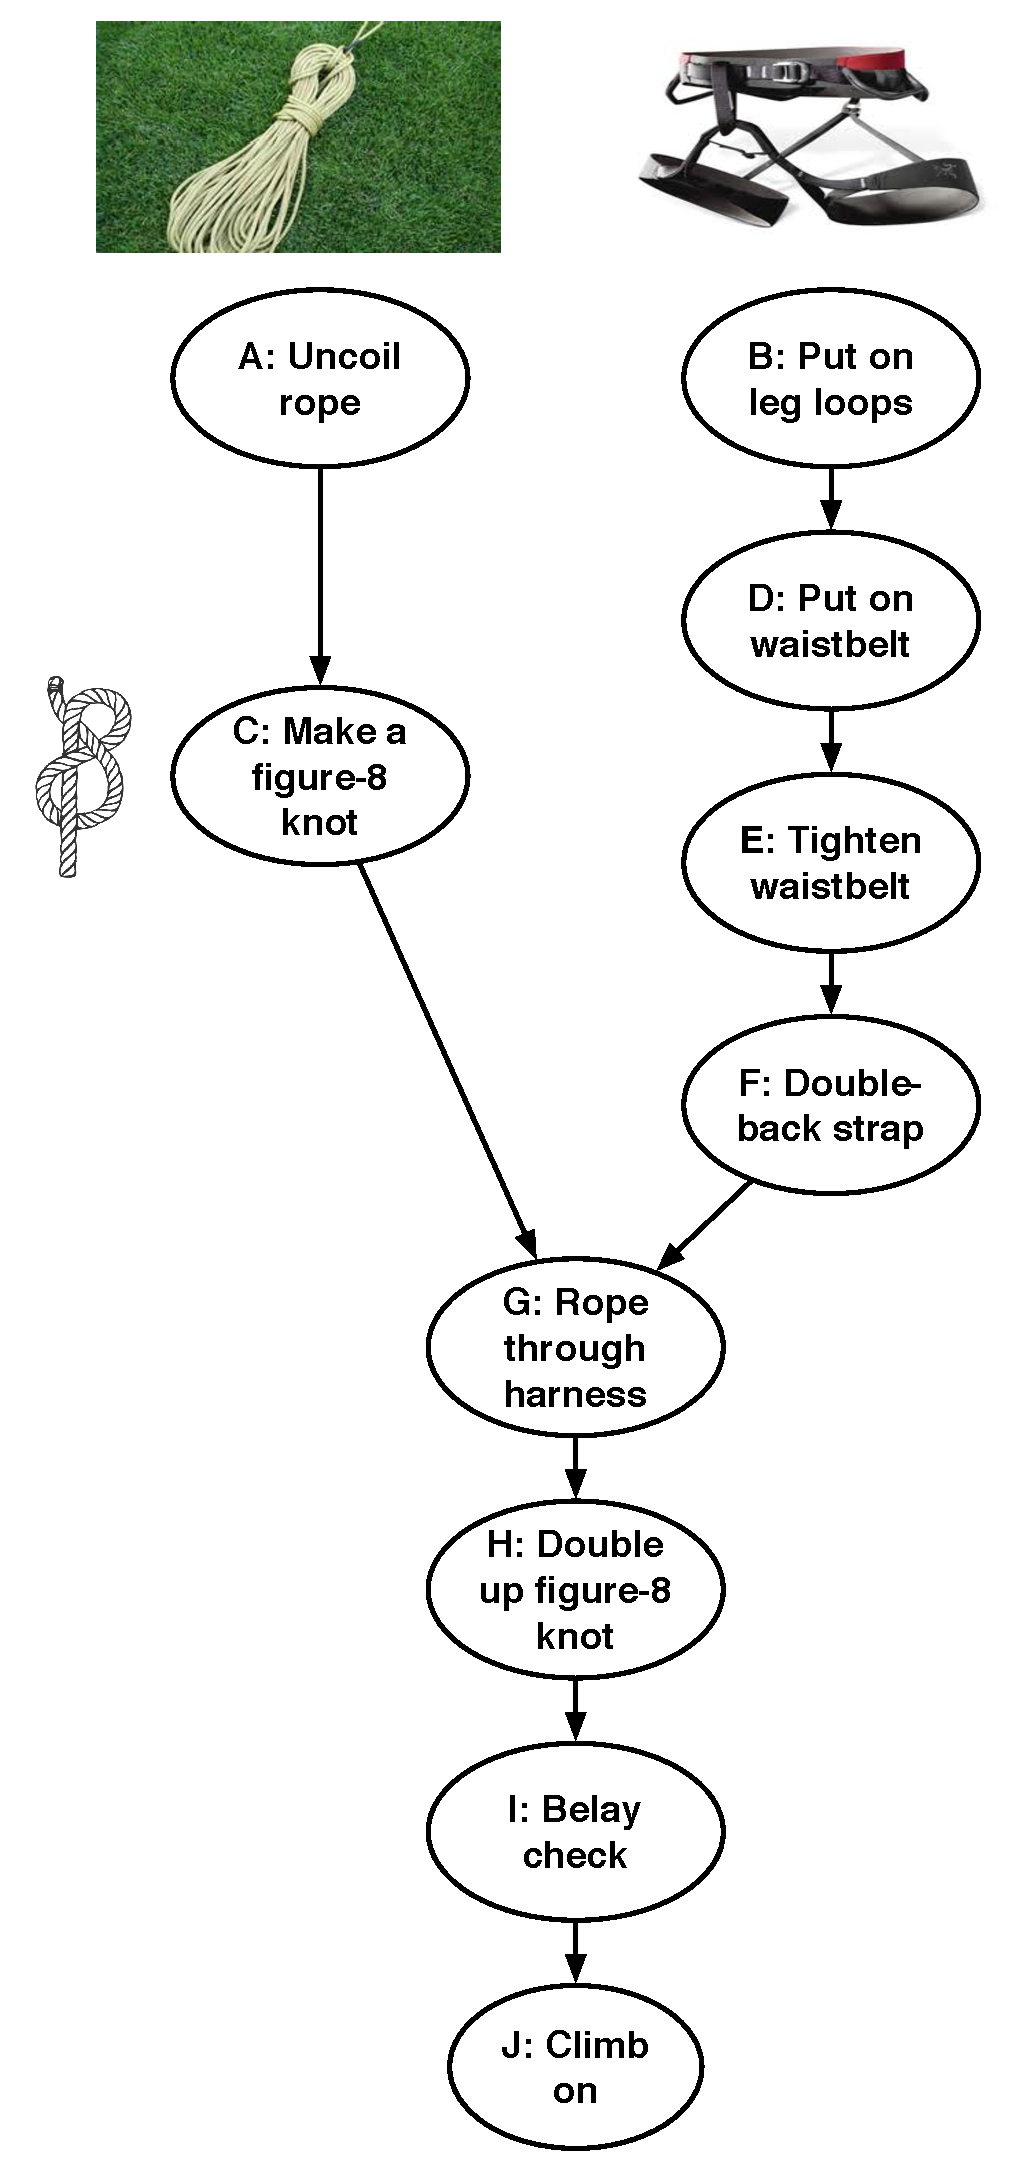
\includegraphics[width=3.5in]{graph-search/climbing-dag}
\end{center}
\caption{A simplified DAG for tying into a rope with a harness.}
\label{fig:dfs::climbing-dag}
\end{figure}

\begin{question}
There is something interesting about the structure of this graph.  Can
you see something missing in this graph compared to a general graph?
\end{question}

Graphs such as these that represents tasks and dependencies between
them are sometimes called \defn{dependency graphs}.
%
An important property of dependency graphs is that they have no
cycles.
%
In general, we refer to a directed graph without cycles as a
\defn{directed acyclic graph} or a \defn{DAG} for short.


Since a climber can only perform one of these tasks at a time (at
least without help), her
actions are naturally ordered. We call a total ordering of the
vertices of a DAG that respects all dependencies a topological sort.

\begin{definition}[Topological Sort of a DAG]
  The topological sort of a DAG $(V,E)$ is a total ordering, $v_1 < v_2
  \ldots < v_n$ of the vertices in $V$ such that for any edge $(v_i,
  v_j) \in E$, we have $v_i < v_j$.
\end{definition}

\begin{question}
Can you come up with a topological ordering of the climbing DAG shown
in \figref{dfs::climbing-dag}.
\end{question}

There are many possible topological orderings for the DAG in
\figref{dfs::climbing-dag}.  For example, following the tasks in
alphabetical order yield a topological sort.  For a climber's
perspective, this is not a good order, because it has too many switches
between the harness and the rope.  
%
To minimize errors, climbers prefer to put on the harness (tasks B, D,
E, F in that order), prepare the rope (tasks A and then C), rope
through, and finally complete the knot, get her gear checked, and
climb on (tasks G, H, I, J, in that order).

\begin{question}
Can you use BFS to compute the topological sort of a graph?
\end{question}

We will soon see how to use DFS as an algorithm to solve topological
sorting.
%
BFS cannot be used to implement topological sort,
because BFS visits vertices in the order of their distance from the
source. This can break dependencies, because dependencies on the
longer paths may be ignored.
%
In our example, the BFS algorithm could ask the climber to rope
through the harness (task G) before fully putting on the harness.


\subsubsection{Depth-First Search (DFS)}

Recall that in graph search, we can choose any (non-empty) subset of
the vertices on the frontier to visit in each round. 
%
The DFS algorithm is a specialization of graph search that picks the
vertex that is most recently added to the frontier.  
%
Intuitively, when a vertex is visited, we can think of ``seeing'' all
the neighbors in some order; the DFS algorithm visits the most
recently seen vertex that is in the frontier (i.e. that has not
already been visited).

\begin{question}
  How can we determine the next vertex to visit?
\end{question}
%
One way to find the most recently seen vertex is to time-stamp the
neighbors when we visit a vertex, and then use these time stamps by
always picking the most recent (largest) one.
%
Since time stamps increase monotonically and since we always visit the
largest one, we can implement this approach by using a stack, which
implicitly keeps track of the ordering of the time-stamps (more recently added vertices are
closer to the top of the stack).
%
We can refine this solution one-more level and implicitly represent
the stack by using recursion.  
%
\algref{dfs::reachability} below defines such an algorithm
based on this idea.
 
\begin{algorithm}[DFS reachability]~
\label{alg:dfs::reachability}
\begin{lstlisting}
reachability $(G,s)$ = 
  let DFS $(X,v)$ =       
       if $v \in X$ then $X$   
       else iterate DFS $(X \cup \{v\})$ $(N_G(v))$ 
  in DFS $(\cset{},s)$ end
\end{lstlisting}
\end{algorithm}

The algorithm maintains a set of visited vertices $X$.  In \ttt{DFS} if the vertex
$v$ has not already been visited, then the algorithms marks it as
visited by adding it to the set $X$ (i.e. $X \cup \cset{v}$), and then
iterates over the neighbors of $v$, running \dfs{} on
each.  
%
The algorithm returns all visited vertices, which is the final value
of $X$. 
As with BFS, this will be the vertices reachable from $s$ (recall that
all graph search techniques we consider identify the reachable vertices).
%
Note, however, that unlike the previous algorithms we have shown
for graph search, the frontier is not maintained explicitly.
Instead
it is implicitly represented in the recursion---i.e., when we return
from DFS, its caller will continue to iterate over vertices in the frontier.

\begin{example}
An example of DFS on a graph where the out-edges are ordered counterclockwise,
starting from the left.

\vspace{-.3in}
\begin{center}
\raisebox{-1.2in}{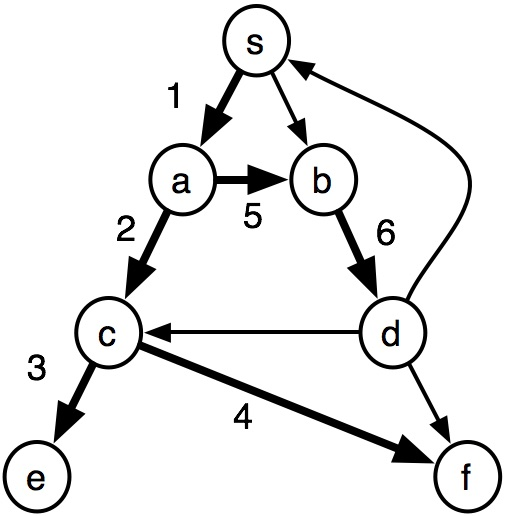
\includegraphics[width=2in]{graph-search/directed-graph-dfs}}
~~~~~~~~~~
$\begin{array}{ll}
v & X  \\ \hline
s & \cset{}  \\
a & \cset{s}  \\
c & \cset{s,a}  \\
e & \cset{s,a,c}  \\
f & \cset{s,a,c,e}  \\
b & \cset{s,a,c,e,f}  \\
d & \cset{s,a,c,e,f,b}  \\
c & \cset{s,a,c,e,f,b,d}  \\
f & \cset{s,a,c,e,f,b,d}  \\
s & \cset{s,a,c,e,f,b,d}  \\
b & \cset{s,a,c,e,f,b,d}  \\
\end{array}
$
\end{center}
Each row corresponds to one call to \ttt{DFS} in
the order they are called, and $v$ and $X$ are the arguments to the
call.   In the last four rows the vertices have
already been visited, so the call returns immediately without
revisiting the vertices since they appear in $X$.
\end{example}

\begin{exercise}
Convince yourself that using generic graph search where the frontier
is represented as a stack visits the vertices in the same order as the
recursive implementation of DFS.
\end{exercise}

The recursive formulation of DFS has an important property---it makes
it easy not just to identify when a vertex is first visited (i.e.,
when adding $v$ to $X$), but also to identify when everything that is
reachable from $v$ has been visited, which occurs when the
\ttt{iterate} completes.
%
As we will see, many applications of DFS require us to do something at
each of these points.


\begin{notesonly}
\begin{figure}
\begin{center}
\includegraphics[width=4.5in]{graph-search/hansel-and-gretel-rackham}
\end{center}
\caption{The idea of pebbling is old.  In H\"ansel and Gretel, one of
  the folk tales collected by Grimm brothers in early 1800's, the
  protagonists use (white) pebbles to find their way home when left in
  the middle of a forest by their struggling parents.  In a later
  adventure, they use bread crumbs instead of pebbles for the same
  purpose (but the birds eat the crumbs, leaving their algorithm
  ineffective).  They later outfox a witch and take possession of all
  her wealth, with which they live happily ever after.  Tales such as
  H\"ansel and Gretel were intended to help with the (then fear-based)
  disciplining of children.  
%Consider the ending though---so much for scare tactics.
}
\label{fig:dfs::hansel-and-gretel}
\end{figure}
\end{notesonly}




\section{DFS Numbers and the DFS Tree}
Applications of DFS usually require us to perform some computation at
certain points during search.  
%
To develop some intuition for the structure of DFS and the important
points during a DFS, think of curiously browsing photos of your
friends in a photo sharing site.
%
For the purposes of this exercise, let's suppose that you have a list
of your friends in front of you and also a bag of colorful pebbles.
%
You start by visiting the site of a friend and put a white pebble next
to his name to remember that you have visited their site.
%
You then realize that some other friends are tagged in your friend's
photos, so you visit the site of one, marking again their name with a
white pebble.
%
Then in that new site, you see other friends tagged and visit the site
of another and again pebble their name white.  
%
Of course, you are careful not to revisit friends that you have
already visited, which are easily noticeable thanks to the pebbles. 
%
When you finally reach a site that contains no one you know that you
have not already visited, you are
ready to press the back button.  
%
However, before you press the back button you change the pebble for
that friend from white to red to indicate that you have completely
explored their site and everything reachable from them.  
%
You then press the back button, which moves you to the site you
visited immediately before first visiting the current one (also the
most recently visited site that still has a white pebble on it). 
%
You now check if another friend that you have not visited is tagged on
that site.  
%
If there is, you visit and so on.
%
When done visiting all neighbors you change that site from a white to
a red pebble, and hit the back button again.  This continues until you
change the site of your original friend from a white pebble to a red
pebble.
%
This process of turning a vertex white and then later red is a
conceptual way to identify two important points in the search. 

To make precise this notion of turning a vertex white and red in DFS,
we can assign two timestamps to each vertex.  The time at which a
vertex receives its white pebble is called the \defn[discovery time in
DFS]{discovery time}.  The time at which a vertex receives its red
pebble is called \defn[finishing time in DFS]{finishing time}.  We
refer to the timestamps as \defn{DFS numbers}.    

\begin{example}
\label{ex:dfs::pebbles}
A graph and its DFS numbers illustrated; $t_1/t_2$ denotes the
timestamps showing when the vertex gets its white (discovered) and red
pebble (finished) respectively.
\begin{center}
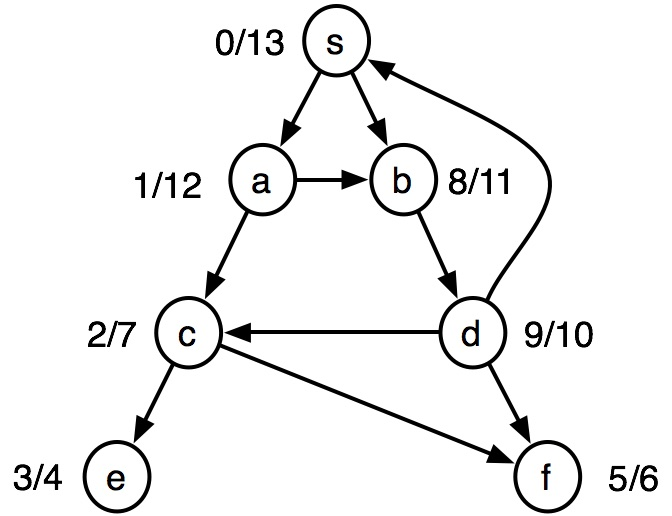
\includegraphics[scale=.55]{graph-search/directed-graph-pebbles}
\end{center}
Note that vertex $\vname{a}$ gets a finished timed of $12$ since it
does not finish until everything reachable from its two out neighbors,
$c$ and $b$, have been fully explored.  Vertices $\vname{d}$,
$\vname{e}$ and $\vname{f}$ have no un-visited out neighbors, and hence
their finishing time is one more than their discovery time.
\end{example}

Given a graph and a DFS of the graph, it is can be useful to classify
the edges of into categories as follows.

\begin{definition}[Tree and Non-Tree Edges in DFS] 
We call an edge $(u,v)$ a {\em tree edge} if $v$ receives its white
pebble when the edge $(u,v)$ was traversed.  Tree edges define the
{\em DFS tree}, which is a special case of a graph-search tree for DFS.
%
The rest of the edges in the graph, which are non-tree edges, can
further be classified as back edges, forward edges, and cross edges.
\begin{itemize}
\item 
A non-tree edge $(u,v)$ is a {\em back edge} if $v$ is an ancestor of
$u$ in the DFS tree.

\item
A non-tree edge $(u,v)$ is a {\em forward edge} if $v$ is a descendant
of $u$ in the DFS tree.

\item
A non-tree edge $(u,v)$ is a {\em cross edge} if $v$ is neither an
ancestor nor a descendant of $u$ in the DFS tree.
\end{itemize}
\end{definition}


\begin{example}
Tree edges (black), and non-tree edges (red, dashed) illustrated with
the original graph and drawn as a tree.  

\begin{center}
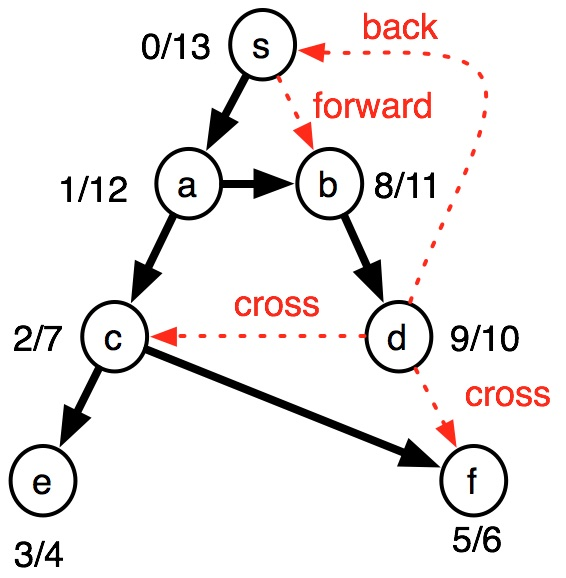
\includegraphics[scale=.55]{graph-search/directed-graph-dfs-tree}
~~~~~~~
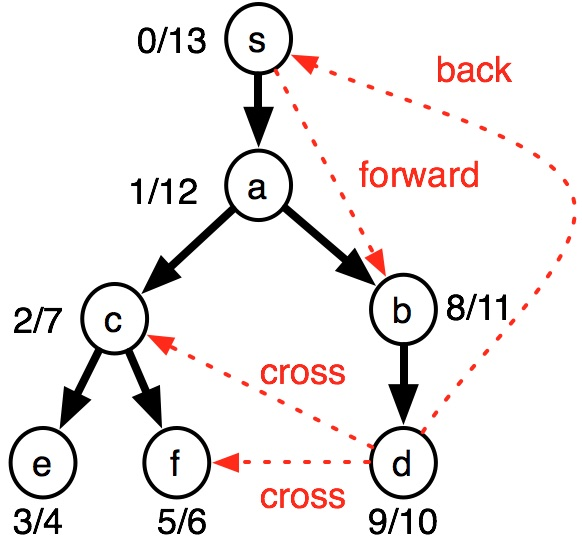
\includegraphics[scale=.55]{graph-search/directed-graph-dfs-tree-rooted}
\end{center}
\label{ex:dfs::dfs-tree}
\end{example}


\newcommand{\revisit}{\ttt{revisit}}
\newcommand{\discover}{\ttt{discover}}
\newcommand{\finish}{\ttt{finish}}

\begin{exercise}
How can you determine by just using the DFS numbers of the endpoints
of an edge whether it is a cross edge, forward edge, or backward edge?
\end{exercise}

\begin{question}
Can you think of a way to implement pebbling efficiently? 
\end{question}

It also useful to consider the point at which we \defn[revisit in
DFS]{revisit} a vertex in DFS and find that it has already been
visited.     We can rewrite our DFS algorithm
(\algref{dfs::reachability}) so that the discover, finish and revisit
times are made clear as follows.

\begin{algorithm}[DFS with discover, finish and revisit]~
\begin{lstlisting}
reachability $(G,s)$ = 
  let DFS $(X,v)$ =       
    if $v \in X$ then $X$  % revisit $v$
    else let
      $X'$ = $X \cup \{v\}$  % discover and visit $v$
      $X''$ = iterate DFS $(X \cup \{v\})$ $(N_G(v))$ 
    in $X''$  % finish $v$
  in DFS $(\cset{},s)$ end
\end{lstlisting}
\end{algorithm}

\begin{notesonly}
We can write a version of DFS that corresponds closely to the DFS
numbers, making explicit the points at which a vertex is discovered,
finished, and revisited (if any).  Viewing DFS in this way helps in
applying the technique to solve different problems.  In fact, later in
this chapter we describe a higher-order version of DFS that can be
used to solve different problems by simply instantiating it with
different arguments.  

\begin{algorithm}[Time-Stamping DFS]
~\\
\begin{lstlisting}
TimeStampingDFS $(G,s)$ = 
  let
    DFS $((X,t),v)$ =
      if $v \in X$ then 
        (* Revisit $v$ *)
        $(X,t)$ 
      else
        let
          (* Discover and Visit $v$ *)
          $td$ = $t + 1$
          $X'$ = $X \cup \{(v,td,\bot)\}$ 
          $(X'',t')$ =  iter DFS $(X',td)$ $(N^+_G(v))$ 
          (* Finish $v$ *)
          $tf$ = $t'+1$
          $X'''$ = $X'' \setminus \{(v,td,\bot)\} \cup \{(v,td,tf)\}$ 
        in
          $(X''',tf)$ 
        end
  in 
    DFS $((\emptyset,-1),s)$ 
  end
\end{lstlisting}
\end{algorithm}
\end{notesonly}


\section{Applications of DFS}

We now consider three applications of DFS: topological sorting (as
introduced earlier), finding cycles in undirected graphs and finding
cycles in directed graphs.    These applications make use of
the categorization of edges, the DFS numbering and the notion
of discovering, finishing and revisiting.


\subsubsection{Topological sorting}

The DFS numbers have many interesting properties.  One of these
properties, established by the following lemma, makes it possible to
use DFS for topological sorting.


\begin{lemma}
  When running DFS on a DAG, if a vertex $u$ is reachable from $v$
  then $u$ will finish before $v$ finishes.
\begin{proof}
  This lemma might seem obvious, but we need to be a bit careful.
  We consider two cases.
\begin{enumerate}
\item $u$ is discovered before $v$.   In this case $u$ must
finish before $v$ is discovered otherwise there would be a
path from $u$ to $v$ and hence a cycle.
\item $v$ is discovered before $u$.  In this case since $u$ is
  reachable from $v$ it must be visited while searching from $v$ and
  therefore finish before $v$ finishes.
\end{enumerate}
\vspace{-.3in}
\end{proof}
\end{lemma}


Intuitively, the lemma holds because DFS fully searches any un-visited
vertices that are reachable from a vertex before returning from that
vertex (i.e., finishing that vertex). 
%
This lemma implies that if we order the vertices by finishing time
(latest first), then all vertices reachable from a vertex $v$ will
appear after $v$ in the ordering, since they must finish before $v$
finishes.  This is exactly the property we require from a topological
sort.

\begin{figure}
\begin{algorithm}[Topological Sort]~
\label{alg:topsort}
\begin{lstlisting}
topSort $(G=(V,E))$ = 
  let DFS $((X,\underline{S}),v)$ = 
      if $v \in X$ then
        $(X,\underline{S})$  % Revisit $v$
      else 
        let
          $X' = X \cup \{v\}$                        % Discover $v$ @\label{line:topsort:discover}@
          $(X'',\underline{S'})$ = iterate DFS $(X',\underline{S})$ $(N_G^+(v))$ 
        in $(X'', \underline{\ttt{cons}(v,S')})$ end                 % Finish $v$ @\label{line:topsort:finish}@ @\vspace{.1in}@
  in second (iterate DFS $(\{\},\underline{\cseq{}})$ $V$) end
\end{lstlisting}
\end{algorithm}
\end{figure}

Algorithm~\ref{alg:topsort} gives an implementation of topological
sort.  Instead of generating DFS numbers, and sorting them, which is a
bit clumsy, it maintains a sequence $S$ and whenever finishing a
vertex $v$, appends $v$ to the front of $S$, i.e. \ttt{cons}$(v,S)$.
This gives the same result since it orders the vertices by reverse
finishing time.  The main difference from the \ttt{reachability}
version of \dfs{} is that we thread the sequence $S$, as indicated by
the underlines.  In the code we have marked the discovery
(Line~\ref{line:topsort:discover}) and finish points
(Line~\ref{line:topsort:finish}).  The vertex is added to the front of
the list at the finish.  
%
The last line iterates over all the vertices
to ensure they are all included in the final topological sort.
%
Alternatively we could have added a ``start'' vertex and an edge from
it to every other vertex, and then just searched from the start.  The
algorithm just returns the sequence $S$ (the second value), throwing
away the set of visited vertices $X$.

\subsubsection{Cycle Detection in Undirected Graphs}

The second problem we consider is determining if there are cycles
in an undirected graph.   Given a graph $G =
(V, E)$ the  \emph{cycle detection} problem is to determine if there are
any cycles in the graph.  The problem is different depending on
whether the graph is directed or undirected.  We first consider
the undirected case, and then the directed case.

How would we modify the generic \dfs{} algorithm above to solve this
problem?  A key observation is that in an undirected graph if $\dfs'$
ever arrives at a vertex $v$ a second time, and the second visit is
coming from another vertex $u$ (via the edge $(u,v)$), then there must
be two paths between $u$ and $v$: the path from $u$ to $v$ implied by
the edge, and a path from $v$ to $u$ followed by the search between
when $v$ was first visited and $u$ was visited.  Since there are two
distinct paths, there is a ``cycle''.  Well not quite!  Recall that in
an undirected graph a cycle must be of length at least 3, so we need
to be careful not to consider the two paths $\cseq{u,v}$ and
$\cseq{v,u}$ implied by the fact the edge is bidirectional (i.e. a
length 2 cycle).  It is not hard to avoid these length two cycles by
removing the parent from the list of neighbors.
These observations lead to the following algorithm.


\begin{algorithm}[Undirected cycle detection]~
\label{lst:dfs::cycle-undir}
\begin{lstlisting}
undirectedCycle $(G = (V,E))$ = 
  let
    $s$ = a new vertex     % used as top level parent @\vspace{.1in}@
    DFS $\underline{p}$ $((X,\underline{C}),v)$ =
      if $(v \in X)$ then 
        $(X, \underline{true})$             % revisit $v$
      else 
        let         
          $X'$ = $X \cup \{v\}$      % discover $v$ 
          $(X'', \underline{C'})$ = iterate $(\ttt{DFS}~\underline{v})$ $(X',\underline{C})$ $(N_G(v) \underline{\setminus \{p\}})$
        in $(X'',\underline{C'})$ end        % finish $v$@\vspace{.1in}@
  in second (iterate (DFS $\underline{s}$) $(\cset{},\underline{false})$ $V$) end
\end{lstlisting}
\end{algorithm}

The algorithm iterates over all vertices in the final line in case the
graph is not connected.   It uses a ``dummy'' vertex $s$ as the parent
at the top level.   The key differences from the generic \dfs{} are underlined.
The variable $C$ is a Boolean variable indicating whether a cycle has
been found so far.  It is initially set to \cfalse{} and set to
\ctrue{} if we find a vertex that has already been visited.  The extra
argument $p$ to $\dfs'$ is the parent in the \dfs{} tree, i.e. the
vertex from which the search came from.  It is needed to make sure we
do not count the length 2 cycles.  In particular we remove $p$ from
the neighbors of $v$ so the algorithm does not go directly back to $p$
from $v$.  The parent is passed to all children by ``currying'' using
the partially applied $(\dfs'~v)$.  If the code executes the
\texttt{revisit $v$} line then it has found a path of length at least
2 from $v$ to $p$ and the length 1 path (edge) from $p$ to $v$, and
hence a cycle.

\subsubsection{Cycle Detection in Directed Graphs}

We now consider cycle detection but in the directed case.  This can be
an important preprocessing step for topological sort since topological
sort will return garbage for a graph that has cycles.  Here is the
algorithm:

\begin{algorithm}[Directed cycle detection]~
\label{lst:dfs::cycle-dir}
\begin{lstlisting}
directedCycle $(G=(V,E))$ = 
  let DFS $\underline{Y}$ $((X,\underline{C}),v) = $
      if $(v \in X)$ then 
        $(X,\underline{C \vee Y[v]})$       % revisit $v$
      else let
          $X' = X \cup \{v\}$     % discover $v$
          $\underline{Y' = Y \cup \{v\}}$
          $(X'', \underline{C'}) =$ iterate (DFS $Y'$) $(X',  \underline{C})$ $(N_{G'}(v))$
        in $(X'',\underline{C'})$ end     % finish $v$@\vspace{.1in}@
  in second(iterate (DFS $\cset{}$) $(\{\},\underline{false})$ $V$) end
\end{lstlisting}
\end{algorithm}

The differences from the generic version are once again underlined.
In addition to threading a Boolean value $C$ through the search that
keeps track of whether there are any cycles, it maintains the
set $Y$ of ancestors in the \dfs{} tree.   In particular when visiting a vertex $v$,
and before recursively visiting its neighbors, we add $v$ to the set $Y$.
To see how maintaining the ancestors helps recall that a \emph{back edge} in a \dfs{}
search is an edge that goes from a vertex $v$ to an ancestor $u$ in
the \dfs{} tree.
We can then make use of the following theorem.
\begin{theorem}
  A directed graph $G = (V,E)$ has a cycle if and only if 
  a DFS over the vertices has a back edge.
\end{theorem}
% Note : might want to be more precise about "over the vertices"

\begin{exercise}
Prove this theorem.
\end{exercise}
Our algorithm for directed cycles therefore simply needs to check if
there are any back edges, which is only true if it revisits an
ancestor, i.e., a vertex in $Y$.

\newcommand{\ctouchf}{\ttt{revisit}}
\newcommand{\centerf}{\ttt{discover}}
\newcommand{\cexitf}{\ttt{finish}}

\subsubsection{Higher-Order DFS}

As already described there is a common structure to all the
applications of \dfs{}---they all do their work either when
``discovering'' a vertex, when ``finishing'' it, or when
``revisiting'' it, i.e. attempting to visit when already visited.
This suggests that we might be able to derive a generic version of
\dfs{} in which we only need to supply functions for these three
components.  This is indeed possible by having the user define a state
of type $\alpha$ that can be threaded throughout search, and then
supplying and an initial state and the following three functions.
More specifically, each function takes the state, the current vertex
$v$, and the parent vertex $p$ in the \dfs{} tree, and returns an
updated state.  The \cexitf{} function takes both the discover and the
finish state.  The algorithm for generalized DFS for directed graphs
can then be written as:


\begin{algorithm}[Generalized directed DFS]
~\\
\begin{lstlisting}
directedDFS $(\ctouchf,\centerf,\cexitf)$ $(G,\Sigma_0,s)$ = 
  let
    DFS  $p$ $((X,\Sigma),v)$ =
      if $(v \in X)$ then 
        $(X, \underline{\ctouchf}~(\Sigma,v,p))$
      else
        let
          $\Sigma'$ = $\underline{\centerf}~(\Sigma,v,p)$
          $X' = X \cup \{v\}$
          $(X'',\Sigma'') = $ iterate (DFS $v$) $(X',\Sigma')$ $(N^+_G(v))$@\label{line:genericngh}@
          $\Sigma''' = \underline{\cexitf}~(\Sigma',\Sigma'',v,p)$
        in $(X'',\Sigma''')$ end
  in 
    DFS $s$ $((\emptyset,\underline{\Sigma_0}),s)$ 
  end
\end{lstlisting}
\end{algorithm}

At the end, \dfs{} returns an ordered pair $(X, \Sigma) : \ttt{Set}
\times \alpha$, which represents the set of vertices visited and the
final state $\Sigma$.  The generic search for undirected graphs is
slightly different since we need to make sure we do not immediately
visit the parent from the child.  As we saw this causes problems in
the undirected cycle detection, but it also causes problems in other
algorithms.  The only necessary change to the directedDFS is to
replace the $(N^+_G(v))$ at the end of Line~\ref{line:genericngh} with
$(N^+_G(v) \setminus \cset{p})$.

With this generic algorithm we can easily define our applications of
\dfs{}.  For undirected cycle detection we have:

\begin{algorithm}[Undirected Cycles with generalized undirected DFS]
~\\
\begin{lstlisting}[numbers=none]
$\Sigma_0 =$ false : bool
$\ctouchf(\_)$ = $\ttt{true}$
$\centerf(\ttt{fl},\_,\_)$ = $\ttt{fl}$
$\cexitf(\_,\ttt{fl},\_,\_)$ = $\ttt{fl}$
\end{lstlisting}
\end{algorithm}


For topological sort we have.

\begin{algorithm}[Topological sort with generalized directed DFS]
~\\
\begin{lstlisting}[numbers=none]
$\Sigma_0 = [~] : \ttt{vertex}~\ttt{list}$
$\ctouchf(L,\_,\_)$ = $L$
$\centerf(L,\_,\_)$ = $L$
$\cexitf(\_,L,v,\_)$ = $v::L$
\end{lstlisting}
\end{algorithm}


For directed cycle detection we have.

\begin{algorithm}[Directed cycles with generalized directed DFS]
~\\
\begin{lstlisting}[numbers=none]
$\Sigma_0$ = ($\cset{}$,false) : Set $\times$ bool
$\ctouchf~((S,\ttt{fl}),v,\_)$ = $(S,~\ttt{fl} \vee (S[v]))$
$\centerf~((S,\ttt{fl}),v,\_)$ = $(S \cup \cset{v},\ttt{fl})$
$\cexitf~((S,\_),(\_,\ttt{fl}),v,\_)$ = $(S,\ttt{fl})$
\end{lstlisting}
\end{algorithm}

For these last two cases we need to also augment the graph with the
vertex $s$ and add the edges to each vertex $v \in V$.  Note that
none of the examples actually use the last argument, which is the
parent.  There are other examples that do.


\section{Cost of DFS}
At first sight, we might think that DFS can be parallelized by
searching the out edges in parallel.  This might work if the searches
on each out edge never ``meet up'' as would be the case for a tree.
However, when portions of the graph reachable through the outgoing
edges are shared, visiting them in parallel creates complications.  This
is because it is important that each vertex is only visited
(discovered) once, and in DFS it is also important that the earlier
out-edge discovers any shared vertices, not the later one.
\begin{example}
Consider the example graph drawn below.
\begin{center}
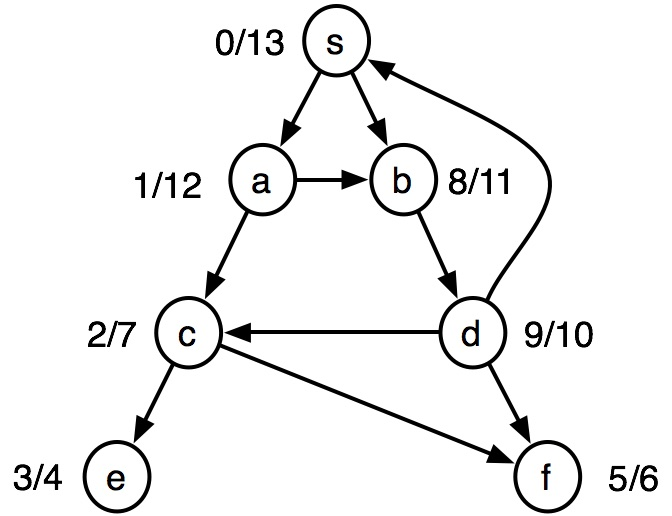
\includegraphics[scale=.55]{graph-search/directed-graph-pebbles}
\end{center}
If we search the out-arcs of $s$ in parallel, we would visit the
vertices $a$, $c$ and $e$ in parallel with $b$, $d$ and $f$.  
%
This is not the DFS order because in the DFS order $b$ and $d$ will be
visited after $a$.  In fact, it is BFS ordering.  
%
Furthermore the two parallel searches would have to synchronize to
avoid visiting vertices, such as $b$, twice.
\end{example}

\begin{remark}
Depth-first search is known to be $\PCLASS$-complete, a class of
computations that can be done in polynomial work but are widely
believed not to admit a polylogarithmic span algorithm.  A detailed
discussion of this topic is beyond the scope of this book, but it
provides evidence that DFS is unlikely to be highly parallel.
\end{remark}

We therefore assume there is no parallelism in DFS and focus on the
work.  The work required by DFS will depend on the data structures
used to implement the set, but generally we can bound work by counting
the number of operation and multiplying this count by the cost of each
operation.  In particular we have the following lemma.

\begin{lemma}
  For a graph $G = (V,E)$ with $m$ edges, and $n$ vertices, \ttt{DFS}
  function in \algreftwo{dfs::reachability}{topsort} will be called at
  most $n+m$ times and a vertex will be discovered (and finished) at
  most $n$ times.
\begin{proof}
  Since each vertex is added to $X$ when it is first discovered, every
  vertex can only be discovered once.  It follows that every out edge
  will only be traversed once, invoking a call to \dfs{}.  Therefore
  \dfs{} is called at most $m$ times through an edge.  In topological
  sort, an additional $n$ initial calls are made starting at each
  vertex.
\end{proof}
\end{lemma}

Each call to \dfs{} performs one find for $X[v]$.  Every time the
algorithm discovers a vertex, it performs one insertion of $v$ into
$X$.  In total, the algorithm therefore performs at most $n$
insertions and $m+n$ finds.  This results in the following cost
specification.

\begin{costspec}[DFS]
  The $\dfs$ algorithm on a graph with $m$ out edges, and $n$
  vertices, and using the tree-based cost specification for sets runs
  in $O((m+n) \log n)$ work and span.  Later we will consider a
  version based on single threaded sequences that reduces the work and
  span to $O(n+m)$.
\end{costspec}


\begin{comment}
\subsection{Generalized DFS}

In DFS, depending on the application, it is sometimes useful to do
something when discovering a vertex (putting a white pebble on it),
sometimes when finishing a vertex (putting a red pebble on it), and
sometimes at both points.  Furthermore it is sometimes necessary to do
something when visiting non-tree edges.  These each correspond to
\emph{revisiting} an already visited vertex.  Based on this observation
we can define a generic version of DFS.  In this version we thread an
application dependent state through the DFS, and the
application supplies functions \discover{}, \finish{}, and \revisit{}
to update this state, if necessary.    These functions also take the vertex,
and the parent in the DFS tree.

\begin{tabular}{lcp{4in}}
\discover$(S,v,p)$ & : & $v$ is the
vertex being discovered, $p$ is its parent in the DFS,
and $S$ is the state when discovered.\\[.1in]

\finish$(S_1,S_2,v,p)$ & : & $S_1$ is the state when
the vertex $v$ was discovered, and $S_2$ is the state after visiting its
neighbors.\\[.1in]

\revisit$(S,v,p)$ & : & $S$ is
the state when the vertex $v$ is revisited, and $S_2$ is the state after
visiting the neighbors.
\end{tabular}

\begin{figure}
\begin{algorithm}[Generalized directed DFS]~
\label{alg:directeddfs}
\begin{lstlisting}
directedDFS ($\Sigma$,discover,finish,revisit) $(G,s)$ = 
let
  DFS $p$ $((X,\Sigma),v)$ =                        % $p$ is the parent
    if $X[v]$ then $(X, \underline{\ctouchf}(\Sigma,v,p))$                  % already visited
    else let
       $\Sigma'$ = $\underline{\centerf}(\Sigma,v,p)$                    % discover
       $(X',\Sigma'') = $ iter (DFS $v$) $(X \cup \{v\},\Sigma')$ $(N^+_G(v))$@\label{line:genericdfsngh}@ % visit neighbors
       $\Sigma''' = \underline{\cexitf} (\Sigma',\Sigma'',v,p)$                   % finish
     in $(X',\Sigma''')$ end@\vspace{.1in}@                      
in DFS $s$ $((\emptyset,\underline{\Sigma}),s)$ end
\end{lstlisting}
\end{algorithm}
\end{figure}

Algorithm~\ref{alg:directeddfs} gives our generic algorithms for DFS.
There are some important things to notice about the code.  Firstly,
the initial state is given by $\sigma$, and this state is threaded
along with the visited set $X$ through the DFS in a sequential order.
Secondly, the DFS takes the parent as an argument.  This is important
since some applications of DFS need to know the parent, as we will
see.  On line~\ref{line:genericdfsngh} the (\ttt{DFS} $v$) partially
applies \ttt{DFS} to the vertex $v$, making it a parent for each of
the recursive calls.

The first example we give is labeling the vertices with their DFS
numbering:
\begin{lstlisting}
DFSNumbering $(G,s)$ = 
let
  $\Sigma$ = $(1, \cset{}, \cset{})$
  dis$((i,W,R),v,\_)$   = $(i+1, W \cup \cset{v \mapsto i}, ~~~~R~~~)$ % add to white
  fin$(\_,(i,W,R),v,\_)$ = $(i+1, ~~~~W~~~~, R \cup \cset{v \mapsto i})$ % add to red
  rev$(S,\_,\_)$ = S         % do nothing
in directedDFS ($\Sigma$,dis,fin,rev) $(G,s)$ end
\end{lstlisting}

\begin{lstlisting}
bridges$(G,s)$ = let
  $\Sigma$ = $(0, \cset{}, \infty, \cset{})$
  discover$((i,W,m_1,B),v,\_)$ =
    let finish$(\_,\_,m_2,B)$ = ($i, W, \min(m_1,m_2)$, 
           if $(m_2 < i)$ then $B \cup \cset{(v,p)}$ else $B$)
    in (finish, $(i+1, W \cup \cset{v \mapsto i}, \infty, B)$) end
  revisit$((\_,\_,W,\_),v,\_)$ = $W[v]$         
in directedDFS ($\Sigma$,discover,revisit) $(G,s)$ end
\end{lstlisting}
\end{comment}

\begin{comment}
\subsection{Topological Sorting}

We now return to topological sorting as a second application of \dfs{}.

\paragraph{Directed Acyclic Graphs.} A directed graph that has no cycles is
called a \emph{directed acyclic graph} or DAG.  DAGs have many important
applications.  They are often used to represent dependence constraints of some
type.  Indeed, one way to view a parallel computation is as a DAG where the
vertices are the jobs that need to be done, and the edges the dependences
between them (e.g. $a$ has to finish before $b$ starts).  Mapping such a
computation DAG onto processors so that all dependences are obeyed is the job of
a scheduler.  You have seen this briefly in 15-150.  The graph of dependencies
cannot have a cycle, because if it did then the system would deadlock and not be
able to make progress.

The idea of topological sorting is to take a directed graph that has
no cycles and order the vertices so the ordering respects
reachability.  That is to say, if a vertex $u$ is reachable from $v$,
then $v$ must be lower in the ordering.  In other words, if we think
of the input graph as modeling dependencies (i.e., there is an edge
from $v$ to $u$ if $u$ depends on $v$), then topological sorting finds
a partial ordering that puts a vertex \emph{after} all vertices that
it depends on.

To make this view more precise, we observe that a DAG defines a
so-called \emph{partial order} on the vertices in a natural way:
\begin{quote}
  For vertices $a, b \in V(G)$, $a \leq_p b$ if and only if there is a
  directed path from $a$ to $b$\footnote{We adopt the convention that
    there is a path from $a$ to $a$ itself, so $a \leq_p a$.}
\end{quote}

Remember that a partial order is a relation $\leq_p$ that obeys
\begin{enumerate}[topsep=0pt,itemsep=1pt]
\item reflexivity --- $a \leq_p a$,
\item antisymmetry --- if $a \leq_p b$ and $b
  \leq_p a$, then $b = a$, and
\item transitivity --- if $a \leq_p b$ and $b
  \leq_p c$ then $a \leq_p c$.
\end{enumerate}

In this particular case, the relation is on the vertices. It's not
hard to check that the relation based on reachability we defined
earlier satisfies these $3$ properties.
Armed with this, we can define the topological sorting problem
formally as follows.

\begin{problem}[Topological Sorting(\probName{TopSort})]
%
  A \emph{topological sort} of a DAG is a total ordering $\leq_t$ on
  the vertices of the DAG that respects the partial ordering (i.e. if
  $a \leq_p b$ then $a \leq_t b$, though the other direction needs not
  be true).
\end{problem}

For instance, consider the following DAG:
\begin{center}
  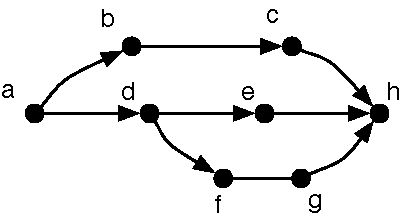
\includegraphics[scale=.75]{graph-search/topsort-1}
\end{center}
We can see, for example, that $a \leq_p c$, $d \leq h$, and $c \leq
h$. But it is a partial order: we have no idea how $c$ and $g$
compare.  From this partial order, we can create a total order that
respects it.  One example of this is the ordering $a \leq_t b \leq_t
\leq_t c \leq_t d \leq_t e \leq_t f \leq_t g \leq_t h$.  Notice that,
as this example graph shows, there are many valid topological
orderings.


\paragraph{Solving \probName{TopSort} using \dfs{}.}

%We now return to \dfs{}.  
To topologically sort a graph, we augment
our directed graph $G = (V,D)$ with a new source vertex $s$
and a set of directed edges from the source to every vertex, giving
$G' = (V \cup \cset{s}, E \cup \cset{(s,v) : v \in V})$.
We then run the following variant of \dfs{} on $G'$ starting at $s$.



\begin{algorithm}[Topological Sort]
~\\
\begin{lstlisting}[
label=lst:dfs::topsort
]
topSort $(G=(V,E))$ = 
  let
    DFS $((X,\underline{L}),v)$ = 
      if $(v \in X)$ then $(X,\underline{L})$   
      else let
          $X' = X \cup \{v\}$    % Discover $v$ @\label{line:topsort::enter}@
          $(X'',\underline{L'})$ = iter DFS $(X',\underline{L})$ $(N_G(v))$
        in $(X'', \underline{v::L'})$ end  % Finish $v$ @\label{line:topsort::exit}@ @\vspace{.1in}@
  in  iter DFS $(\{\},\underline{[~]})$ $V$ end
\end{lstlisting}
\end{algorithm}

The significant changes from the generic version of $\ttt{DFS}'$ are
marked with underlines.  In particular we thread a list $L$ through
the search.  The only thing we do with this list is cons the vertex
$v$ onto the front of it when we exit \dfs{} for vertex $v$ (line
\texttt{Exit $v$}).  We claim that at the end, the ordering in the
list returned specifies a topological sort of the vertices, with the
earliest at the front.

\textbf{Why is this correct?}  The correctness crucially follows from
the property that \dfs{} fully searches any un-visited vertices that
are reachable from it before returning.  In particular the following
theorem is all that is needed.

\begin{theorem}
  On a DAG when exiting a vertex $v$ in \dfs{} all vertices reachable
  from $v$ have already exited.
\end{theorem}

\begin{proof}
  This theorem might seem obvious, but we have to be a bit careful.
  Consider a vertex $u$ that is reachable from $v$ and consider the
  two possibilities of when $u$ is entered relative to $v$.
\begin{enumerate}
\item $u$ is entered before $v$ is entered.   In this case $u$ must
also have exited before $v$ is entered otherwise there would be a
path from $u$ to $v$ and hence a cycle.
\item $u$ is entered after $v$ is entered.   In this case
  since $u$ is reachable from $v$ it must be visited while searching $v$
and therefore exit before $v$ exits.
\end{enumerate}
\vspace{-.3in}
\end{proof}

This theorem implies the correctness of the algorithm for topological
sort.  This is because it places vertices on the front of the list in
exit order so all vertices reachable from a vertex $v$ will appear
after it in the list, which is the property we want.
\vspace{-.1in}
\end{comment}



\subsubsection{DFS with Single-Threaded Arrays}

Here is a version of \dfs{} using adjacency sequences for representing the
graph and ST sequences for keeping track of the visited vertices.

\begin{algorithm}[DFS with single threaded arrays]
~\\
\begin{lstlisting}
directedDFS ($G$:(int seq) seq,$\Sigma_0:\alpha$, $s$:int) =
  let
    DFS $p$ (($X$:bool stseq, $\Sigma:\alpha$, $v$:int) =
      if $(X[v])$ then 
        $(X,\ctouchf~(\Sigma,v,p))$
      else 
        let
          $X'$ = STSeq.update $X$ $(v,\ttt{true})$
          $\Sigma' = \centerf~(\Sigma,v,p)$
          $(X'',\Sigma'')$ = iterate (DFS $v$) $(X',\Sigma')$ $(G[v])$
          $\Sigma''' = \cexitf~(\Sigma',\Sigma'',v,p)$
        in $(X'',\Sigma''')$ end @\vspace{.1in}@
    $X_{init}$ = STSeq.fromSeq $\cseqb$ false : $v \in \cseq{0,\ldots,|G|-1}$ $\cseqe$
  in
    DFS $s$ $((X_{init},\Sigma_0), s)$
  end
\end{lstlisting}
\end{algorithm}

If we use an \texttt{stseq} for $X$ (as indicated in the code) then
this algorithm uses $O(m)$ work and span.
%
However if we use a regular sequence, it requires $O(n^2)$ work and
$O(m)$ span.

\begin{exercise}
Convince yourself that the $O(m)$ bound above is correct, e.g., 
not $O(n+m)$.
\end{exercise}

\section{Priority-First Search}

The graph search algorithm that we described does not specify the
vertices to visit next (the set $U$). This is intentional, because
graph search algorithms such as breadth-first search and depth-first
search differ exactly on which vertices they visit next.  
%
Many graph-search algorithms can be viewed as visiting vertices in
some priority order.  To see this, suppose that a graph-search
algorithm assigns a priority to every vertex in the frontier.
%
We can imagine the algorithm assigning a priority to a vertex $v$ when
it inserts $v$ into the frontier. 
%
Now instead of choosing some unspecified subset of the frontier to
visit next, the algorithm picks the highest (or the lowest) priority
vertices.  Effectively we change \lineref{gs::choose} in the
\ttt{graphSearch} algorithm to:
\begin{lstlisting}[numbers=none]
      Choose $U$ @\ttt{as the highest priority vertices in} $F$@
\end{lstlisting}
We refer to such an algorithm as a \emph{priority-first search (PFS)}
or a {\em best-first search}.  The priority order can either be
determined statically (a priori) or it can be generated on the fly by
the algorithm.


Priority-first search is a greedy technique since it greedily selects
among the choices available (the vertices in the frontier) based on
some cost function (the priorities) and never backs up.  Algorithms
based on PFS are hence often referred to as greedy algorithms.  As you
will see soon, several famous graph algorithms are instances of
priority-first search, e.g., Dijkstra's algorithm for finding
single-source shortest paths and Prim's algorithm for finding Minimum
Spanning Trees.


\begin{simpleexample}
How can you use a priority search to explore the web from a start page
so that the web sites that are of higher importance to you are visited
first?


You can use priority search to explore the web in a way that gives
priority to the sites that you are interested in. The idea would to
implement the frontier as a priority queue data structure containing
the un-visited outgoing links based on your interest on the link (which
we assume to be known). You can then choose what page to visit next by
simply selecting the link with the highest priority. After visiting
the page, you would remove it from the priority queue and add all its
un-visited outgoing links to the list with their corresponding priorities.
\end{simpleexample}

\begin{comment}
\subsection{SML Code} 

Here we give the SML code for the generic version of \dfs{} along with the implementation of directed cycle detection and topological sort.

\begin{small}
\verbatiminput{code/dfs.sml}
\verbatiminput{code/cycleCheck.sml}
\verbatiminput{code/topSort.sml}
\end{small}

\newpage
\begin{figure}
\centering
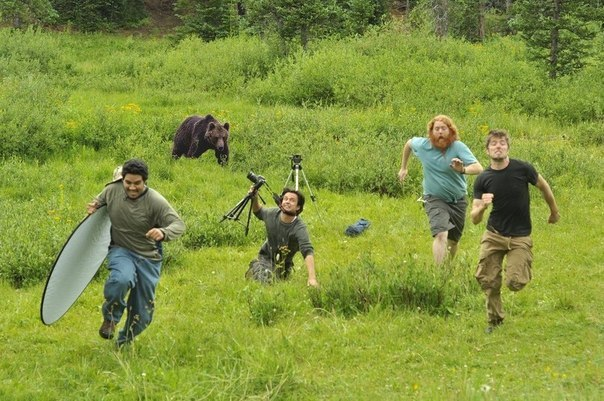
\includegraphics[width=6in]{graph-search/bear}
\caption{Don't forget to have fun.}
\label{fig:dfs::bear}
\end{figure}

\end{comment}

\flushchapter




\flushchapter
